% A basic LaTeX document for a handin with a
% standard RU title page
\newcommand*\rot{\rotatebox{90}}

% If you want the title to appear on a separate
% page, change notitlepage to titlepage
\documentclass{article}
\usepackage[utf8]{inputenc}
\usepackage[T1]{fontenc}
\usepackage[dvipsnames]{xcolor}

\usepackage{fancyvrb}

% redefine \VerbatimInput
\RecustomVerbatimCommand{\VerbatimInput}{VerbatimInput}%
{fontsize=\footnotesize,
 %
 frame=lines,  % top and bottom rule only
 framesep=2em, % separation between frame and text
 rulecolor=\color{Gray},
 %
 label=\fbox{\color{Black}results.csv},
 labelposition=topline,
 %
 commandchars=\|\(\), % escape character and argument delimiters for
                      % commands within the verbatim
 commentchar=*        % comment character
}
% If your hand-in is in icelandic change english to icelandic
% Note: This has nothing to do with Icelandic characters, they
% can always be used. This just tells other packages what
% language you are using and changes the hyphenation used by LaTeX
% If icelandic is selected, a shorthand, "` and "', is also included
% for Icelandic quotation marks. They can also obtained by using
% ,, and ``
\usepackage[icelandic]{babel}
\usepackage{amsmath, amsthm, amssymb, amsfonts}
\usepackage{graphicx}
\usepackage{enumerate}
\usepackage{hyperref}
\usepackage[export]{adjustbox} % Darri
\usepackage{caption} % Darri
\usepackage{subcaption} % Darri
\usepackage[bottom]{footmisc} % Darri
\usepackage{enumitem}

% To use the whole A4-page
% See: ftp://ftp.tex.ac.uk/tex-archive/macros/latex/contrib/geometry/geometry.pdf
% and http://en.wikibooks.org/wiki/LaTeX/Document_Structure
\usepackage[footskip=35pt]{geometry}
% For header and footer
% See: ftp://ctan.tug.org/tex-archive/macros/latex/contrib/fancyhdr/fancyhdr.pdf
% and http://en.wikibooks.org/wiki/LaTeX/Document_Structure
\usepackage{fancyhdr}
% For prettier tables
% See: http://ctan.mackichan.com/macros/latex/contrib/booktabs/booktabs.pdf
% and  http://en.wikibooks.org/wiki/LaTeX/Tables
\usepackage{booktabs}
% Listings allow us to include pretty code in our document
\usepackage{listings}
% A pretty monospace font, will for example appear inside listings and \texttt{}
\usepackage{inconsolata}
\usepackage{pgfplots}
\usepackage{wrapfig}
\usepackage{float}
\usepackage{tabularx}
\usepackage{url}

\definecolor{lb}{RGB}{123,120,219}
\definecolor{lg}{RGB}{102,221,115}
\definecolor{lightgray}{rgb}{.9,.9,.9}
\definecolor{darkgray}{rgb}{.4,.4,.4}
\definecolor{purple}{rgb}{0.65, 0.12, 0.82}


\linespread{1.3}


\usepackage{ifxetex,ifluatex}
\usepackage{etoolbox}
\usepackage{xcolor}

\usepackage{tikz}

\usepackage{framed}
\usepackage{enumitem}

\usepackage{titletoc,tocloft}

%%%%%%%%%%%%%%%%%%%%%%%%%%%%%%%%%%%%%%%%%%%%%%%%%%%%%%%%%%%%%
%                        Setup
%%%%%%%%%%%%%%%%%%%%%%%%%%%%%%%%%%%%%%%%%%%%%%%%%%%%%%%%%%%%%

% Set the margins of the paper. By default LaTeX uses huge margins
\geometry{includeheadfoot, margin=2.5cm}
% you can also use
% \geometry{a4paper}
% End of margins setup

\setlength{\cftsubsecindent}{1cm}
\setlength{\cftsubsubsecindent}{2cm}
\dottedcontents{section}[1.5em]{}{1.3em}{.6em}

\setlist[enumerate]{itemsep=0mm}
\setlist[itemize]{itemsep=0mm}

\lstdefinelanguage{JavaScript}{
  keywords={typeof, new, true, false, catch, function, return, null, catch, switch, var, if, in, while, do, else, case, break, for},
  keywordstyle=\color{blue}\bfseries,
  ndkeywords={class, export, boolean, throw, implements, import, this},
  ndkeywordstyle=\color{darkgray}\bfseries,
  identifierstyle=\color{black},
  sensitive=false,
  comment=[l]{//},
  morecomment=[s]{/*}{*/},
  commentstyle=\color{purple}\ttfamily,
  stringstyle=\color{red}\ttfamily,
  morestring=[b]',
  morestring=[b]"
}

% Fill in any relevant information
% Leave the fields inside the {} empty if they do not apply
\newcommand{\studentA}{Atli Sævar Guðmundsson}
\newcommand{\studentB}{Ægir Már Jónsson}
\newcommand{\studentC}{Darri Ragnarsson}
\newcommand{\studentemailA}{atlisg12@ru.is}
\newcommand{\studentemailB}{aegir13@ru.is}
\newcommand{\studentemailC}{darrir13@ru.is}
\newcommand{\semester}{Vor 2016}
\newcommand{\coursename}{T-404-LOKA, Lokaverkefni}
\newcommand{\ssn}{}
\newcommand{\group}{Rekstrarhandbók 1.04}
\newcommand{\assignment}{Hvert fara peningarnir?}
\newcommand{\division}{B.Sc. Tölvunarfræði}
\newcommand{\university}{Háskólinn í Reykjavík}
\newcommand{\teachingassistant}{Leiðbeinandi: Sigurjón Ingi Garðarsson}
\newcommand{\examiner}{Prófdómari: Daníel Máni Jónsson}
\newcommand{\teacher}{Kennari: Hallgrímur Arnalds}
\newcommand{\problemtitle}{Dæmi}
\newcommand{\solutiontitle}{Lausn}
\newcommand{\programminglanguage}{JavaScript}
\newcommand{\dateofcompilation}{\today}
\newcommand{\code}[5]{\texttt{#5}}

% Setup header and footer
% Headers
\pagestyle{fancy} % To get the header and footer
\rhead{\small \textsc{\group}}
\lhead{\small \textsc{\assignment}}
%\rhead{\small \textsc{\coursename}}
% Footers
%\lfoot{Left footer text}
%\cfoot{\thepage} % This is the default behaviour
%\rfoot{Right footer text}

% If you don't want a line below the header or above the footer,
% change the appropriate header/footerrulewidth to 0pt
\setlength{\headheight}{15.2pt} % This is set to avoid a warning
\setlength{\headsep}{30pt}
\renewcommand{\headrulewidth}{0.4pt}
\renewcommand{\footrulewidth}{0.4pt}
% End of header and footer setup

% Setup Problem/Solution environments
\newtheoremstyle{blueP}{}{}{}{}{\color{orange}\bfseries}{}{ }{}
\theoremstyle{blueP}
\newtheorem{problem}{\problemtitle}

\newtheoremstyle{greenS}{}{}{}{}{\color{lg}\bfseries}{}{ }{}
\theoremstyle{greenS}
\newtheorem*{solution}{\solutiontitle}
% Custom problem (so you can provide the problem name)
\newenvironment{cproblem}[1]{\begin{trivlist}
\item[\hskip \labelsep {\bfseries \problemtitle}\hskip \labelsep {\bfseries#1.}]\begin{itshape}}{\end{itshape}\end{trivlist}}
% End of Problem/Solution environments setup

\usepackage{color}

\definecolor{mygreen}{rgb}{0,0.6,0}
\definecolor{mymauve}{rgb}{0.58,0,0.82}
\definecolor{lightgray}{gray}{0.95}
\definecolor{turquoise}{rgb}{64,224,208}

%\usepackage{xcolor}

%\pagecolor[rgb]{0.15,0.15,0.15}
%\color[rgb]{0.9,0.9,0.9}
\hyphenchar\font=-1
% Feel free to edit these yourself
\lstset{ %
  backgroundcolor=\color{lightgray},   % choose the background color; you must add \usepackage{color} or \usepackage{xcolor}
  rulecolor=\color{turquoise},
  language=JavaScript,   % Set
  basicstyle=\ttfamily,        % the size of the fonts that are used for the code
  breakatwhitespace=false,         % sets if automatic breaks should only happen at whitespace
  breaklines=true,                 % sets automatic line breaking
  captionpos=b,                    % sets the caption-position to bottom
  commentstyle=\color{mygreen},    % comment style
  deletekeywords={...},            % if you want to delete keywords from the given language
  escapeinside={\%*}{*)},          % if you want to add LaTeX within your code
  extendedchars=true,              % lets you use non-ASCII characters; for 8-bits encodings only, does not work with UTF-8
  frame=single,                    % adds a frame around the code
  keepspaces=true,                 % keeps spaces in text, useful for keeping indentation of code (possibly needs columns=flexible)
  columns=fixed,
  keywordstyle=\color{red},       % keyword style
  morekeywords={*,...},            % if you want to add more keywords to the set
  numbers=left,                    % where to put the line-numbers; possible values are (none, left, right)
  numbersep=7pt,                   % how far the line-numbers are from the code
  numberstyle=\ttfamily, % the style that is used for the line-numbers
  showspaces=false,                % show spaces everywhere adding particular underscores; it overrides 'showstringspaces'
  showstringspaces=false,          % underline spaces within strings only
  showtabs=false,                  % show tabs within strings adding particular underscores
  stringstyle=\color{mymauve},     % string literal style
  tabsize=2,                       % sets default tabsize to 2 spaces
  title=\lstname                   % show the filename of files included with \lstinputlisting; also try caption instead of title
}
\lstMakeShortInline[basicstyle=\small\ttfamily\color{cyan}]|


        % Add the title page command
        \newcommand{\maketitlepage}[1]
        {
            \begin{titlepage}

                \begin{center}
                    \includegraphics[width=0.25\textwidth]{./RU_logo}\\[1.0cm]
                    \textsc{\Large \semester}\\[0.1cm]
                    \textsc{\Large \division}\\[0.1cm]
                    \textsc{\Large \coursename}\\[1.0cm]
                    
                    \text{\Large Í samstarfi við Kópavogsbæ}\\[0.3cm]
                    \textsc{\huge \assignment}\\[1.8cm]
                    
                    \textsc{\text{\Huge \group}}\\[1.8cm]
                    
                    \textsc{\Large \teacher}\\[0.1cm]
                    \textsc{\Large \teachingassistant}\\[0.1cm]
                    \textsc{\Large \examiner}\\[1.2cm]
                    
                    \textsc{\large \studentB, }\text{\large \studentemailB}\\
                    \textsc{\large \studentA, }\text{\large \studentemailA}\\
                    \textsc{\large \studentC, }\text{\large \studentemailC}\\[1.2cm]

                    \text{\Large \dateofcompilation}



                \end{center}

                \vfill
            \end{titlepage}
        }
        \newcommand{\command}[1]{\texttt{\textbackslash{}\verb !#1}}
\setcounter{tocdepth}{4}
\setcounter{secnumdepth}{4}
        %%%%%%%%%%%%%%%%%%%%%%%% END OF SETUP %%%%%%%%%%%%%%%%%%%%%%%%


\begin{document}
% Create the title page
    \maketitlepage{\assignment}

\tableofcontents
\clearpage

\section{\Large Inngangur}
Farið verður yfir hvernig allt kerfið virkar, hvernig á að setja það upp og hvernig á að uppfæra gögnin. Fyrst koma notkunarleiðbeiningar fyrir umsjónarmenn kerfisins, þvínæst forritunarreglur verkefnisins, þá verður fjallað um hvernig skal eiga samskipti við vefþjónustuna okkar og að lokum hvernig á að setja allt kerfið upp á hreina þróunarvél, sýndarvél á Azure, ElasticSearch gagnagrunn á henni og Jenkins sjálfkeyrsluumhverfis- vefþjónustutólið.

\section{\Large Notendaleiðbeiningar fyrir umsjónarmenn}
% TODO: Sýna hvernig maður skráir sig inn og uppfærir gagnagrunninn.
Til að uppfæra gagnagrunninn þarf notandinn að skrá sig inn \href{http://hfp.kopavogur.is/#/admin}{hér}.\footnote{http://hfp.kopavogur.is/\#/admin} 
Þar birtist innskráningarsýn (Sjá mynd \ref{fig:adminLogin}). Eftir að notandinn skráir sig inn og innskráning tókst kemur upp forsíða sem hefur aðeins tvo valmöguleika; uppfæra gögn eða útskrá. (Sjá mynd \ref{fig:admin_signed_in}). Þegar ýtt er á að uppfæra gögn er hægt að velja hvaða ár notandinn vill uppfæra (Sjá mynd \ref{fig:admin_update}). Þá koma upp skilaboð sem tilkynna að uppfærslan sé hafin (Sjá mynd \ref{fig:admin_update_started}) og sent er póst á netfang innskráðs stjórnanda með sömu skilaboðum. Ef að uppfærslan misheppnast þá fær notandinn póst á netfangið sitt sem tilkynnir honum að eitthvað hafi farið úrskeiðis annars  heppnaðist uppfærslan og þá er sendur póstur sem lætur vita að uppfærslan hafi tekist. Allt ferlið ætti að taka u.þ.b. 10 mín að uppfæra gagangrunninn á www.hfp.kopavogur.is. 


Kerfið sendir upplýsingarnar á 
\href{http://www.hfp.firebaseio.com}{Firebase}.\footnote{http://www.hfp.firebaseio.com}
sem er með innbyggða virkni til að auðkenna notendur sem sendir token til baka ef netfangið er til í gagnagrunninum og lykilorðið sé rétt. Þannig getum við nýtt okkur að við þurfum bara að útfæra framendann og tengingu við Firebase, en síðan búið til og eytt notendum með Firebase.

% \clearpage

\begin{figure}[H]
\centering
\begin{minipage}{.5\textwidth}
  \centering
  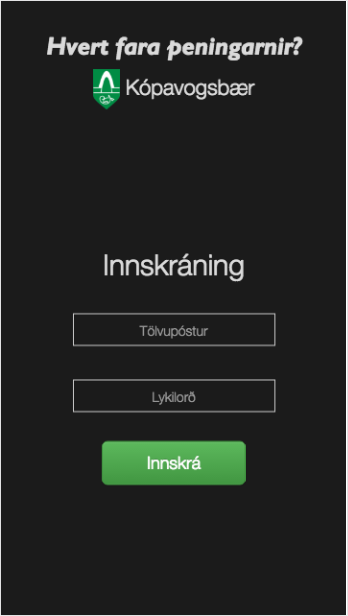
\includegraphics[width=.6\linewidth]{./Admin_login.png}
  \captionof{figure}{Innskráning stjórnanda}
  \label{fig:adminLogin}
\end{minipage}%
\begin{minipage}{.5\textwidth}
  \centering
  
\includegraphics[width=.6\linewidth]{./Admin_signed_in.png}
  \captionof{figure}{Forsíða eftir innskráningu}
  \label{fig:admin_signed_in}
\end{minipage}
\end{figure}

\begin{figure}[H]
\centering
\begin{minipage}{.5\textwidth}
  \centering
  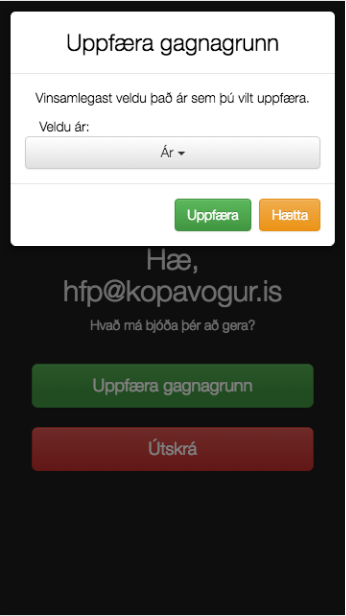
\includegraphics[width=.6\linewidth]{./Admin_update.png}
  \captionof{figure}{Uppfærir eftir ári}
  \label{fig:admin_update}
\end{minipage}%
\begin{minipage}{.5\textwidth}
  \centering
  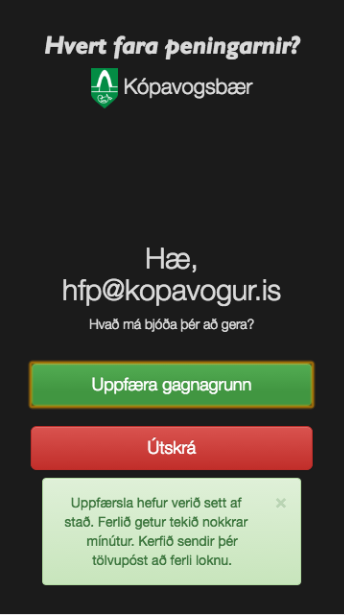
\includegraphics[width=.6\linewidth]{./Admin_Update_started.png}
  \captionof{figure}{Skilaboð tilkynna að ferlið sé farið af stað}
  \label{fig:admin_update_started}
\end{minipage}
\end{figure}

\section{\Large Forritunarreglur}
Þeir sem hyggjast bæta við kóða verkefnisins eru eindregið hvattir til að fylgja forritunarreglum þessum, til að halda kóðanum snyrtilegum, skiljanlegum og samræmdum. Farið verður eftir JavaScript forritunarreglum skrifaðar af Douglas Crockford að hluta til (sjá \url{http://javascript.crockford.com/code.html}). Kóðinn verður skrifaður á ensku og engir sérstafir (æ, ð, þ, é, á...) skulu vera notaðir.

\subsection{Hvít svæði}
Í þessum tilfellum ættu hvít pláss að vera notuð:
\begin{itemize}
    \item Á eftir lykilhugtökum eins og if, else if og while. \\
    \lstinline|while (true)|
    \item Á eftir lykilhugtakinu 'function' skal alltaf koma bil. \\
    \lstinline|var myFunc = function (param1, param2)|
    \item Á eftir öllum kommum ',' skal koma bil eða ný lína.
    \item Á eftir öllum semíkommum ';' á eftir staðhæfingu skal koma ný lína.
    \item Á eftir öllum semíkommum ';' innan 'for' skilgreiningar skal koma bil. \\
    \lstinline|for (i = 0; i < 10; i++)|
    \item Hver inndráttur á að vera á lengd fjögurra bila.
\end{itemize}
Í þessum tilfellum ættu hvít pláss EKKI að vera notuð:
\begin{itemize}
    \item Við fallakall, eftir nafn fallsins og svigans. \\
    \lstinline|myFunc(param1)|
\end{itemize}

\subsection{Umsagnir}
\begin{itemize}
    \item Almennt skrifa umsögn bara í einni línu. \\ \lstinline|i = 0; // Initialize the variable i to zero|
    \item Aðeins nota fjöldalínu umsagnir fyrir formlega skjölun.
    \item Skrifa oftar fremur en sjaldan. Umsagnir eiga að útskýra hvað við erum að gera og af hverju það er gert. 
\end{itemize}

\subsection{Yfirlýsingar á breytum}
\begin{itemize}
    \item Yfirlýsa allar breytur áður en þær eru notaðar.
    \item Forðast að nota óstaðbundnar breytur.
\end{itemize}

\subsection{Yfirlýsingar falla}
\begin{itemize}
    \item Yfirlýsa föll áður en þau eru notuð.
    \item Sleppa því að hafa bil á milli skilgreiningu á falli og vinstri sviga. Hafa bil á milli hægri sviga og slaufusviga. Inndráttur eru fjögur bil og við lokum fallinu með slaufusviga í sama inndrætti og skilgreining fallsins byrjar. \\
    \begin{lstlisting}
    function outer(c, d) {
        var e = c * d;
        return e;
    }\end{lstlisting}
\end{itemize}

\subsection{Nafnagiftir}
\begin{itemize}
    \item Notum 26 stafi í annaðhvort há- og lágstöfum $(A - Z, a -z)$, 10 tölur $(0 - 9)$ og “$\_$” undirstrik.
    \item Við nafnagiftir breytna og falla skal nota lower camel casing, fyrsta orð er allt í lágstöfum og öll orð eftir það hafa stóran upphafsstaf en annars lágstafi, engin bil á milli orða. \\
    \lstinline|var myVariable = 10;| \\
    \lstinline|var myFunc = function() {}|
    \item Við nafnagiftir óstaðbundna breytna (ef notað verður einhverjar) skal nota aðeins hástafi og niðurstrik (\_) á milli orða. \\ 
    \lstinline|var MAX_INT = 1000;|
    \item Við nafnagiftir klasa eða hluta skal nota camel casing, öll orð hafa stóran upphafsstað og hinir stafirnir eru lágstafir. Ekkert bil á milli orða. \\
    \lstinline|var Person = {};|
\end{itemize}

\subsection{Staðhæfingar}
\begin{itemize}
    \item Einfaldar Staðhæfingar:
    \begin{itemize}
        \item Hver lína ætti aðeins að innihalda eina staðhæfingu.
        \item Setjum “;” semíkommu á endann á öllum einföldum staðhæfingum.
    \end{itemize}
    \item Samsettar Staðhæfingar
    \begin{itemize}
        \item Samsettar staðhæfingar eru margar staðhæfingar lokaðar inni í { } slaufusvigum.
        \item Notum sömu reglur og fyrir yfirlýsingu falla. 
        \item Notum slaufusviga fyrir allar staðhæfingar sem eru hluti af röksegðum eða lykkjum, jafnvel þó að þetta sé bara ein ný lína og hægt væri að sleppa slaufusvigunum. 
    \end{itemize}
\end{itemize}

\section{\Large Samskipti við vefþjónustu}
Hægt er að eiga samskipti við vefþjónustuna á \url{http://hfp.northeurope.cloudapp.azure.com:4000} með fjórum mismunandi apaköllum:
\begin{enumerate}
    \item POST beiðni til að uppfæra gagnagrunninn
    \item GET beiðni til að ná í gögn fyrir ``Gjöld''
    \item GET beiðni til að ná í gögn fyrir ``Sameiginlegar tekjur''
    \item GET beiðni til að ná í gögn fyrir ``Sértekjur''
\end{enumerate}

\subsection{Uppfæra gagnagrunn}
Til að uppfæra gagnagrunninn þá þarf að senda POST beiðni á vefþjónustuna með \url{/updateDatabase} með eftirfarandi breytum í body:
\begin{itemize}
    \item year: Árið sem þú vilt uppfæra.
    \item token: Auðkennistákn til að auðkenna notendann.
    \item email: Tölvupóstfang sem þú vilt fá staðfestingarpóst á.
\end{itemize}
Auðkennistáknið verður til við innskráningu umsjónarmanns í stjórnandasýninni \url{/\#/login} í gegnum FireBase og vistast í biðlaranum. Sjá nánar í skjölun biðlara hvernig það ferli fer fram.

Þessi rúta skilar hlut sem inniheldur þrjú eigindi:
\begin{itemize}
    \item updateUnderway: Bool breyta sem segir hvort gagnauppfærslan hafi verið sett í gang eða ekki.
    \item authSuccess: Bool breyta sem segir til um hvort auðkenning hafi tekist eða ekki.
    \item msg: Skilaboðastrengur sem gefur til kynna hvað hafi gerst.
\end{itemize}
    
\subsection{Ná í gögn fyrir gjöld}
Til að ná í gögn fyrir gjöld bæjarins þarf að senda GET beiðni á vefþjónustuna með \\ \url{/expenses/:period/:level/:affairGroupID/:affairID/:divisionGroupID/:divisionID/:financeKeyID/:creditorID}.
\\ Breyturnar eru
\begin{itemize}
    \item period: Tímabil til að skoða. Ef óskað er eftir heilu ári, þá skal senda inn árið með bandstriki og tölustafnum núll. Til að fá ársfjórðung er það alveg eins nema tölustafirnir einn til fjórir á eftir bandstrikinu. Til að fá mánuð þarf að setja tvo tölustafi á eftir bandstrikinu, 01 fyrir janúar, 02 fyrir febrúar ... og 12 fyrir desember. \\ Dæmi:
    \begin{itemize}
        \item 2014-0: Allt árið 2014.
        \item 2015-3: Þriðji ársfjórðungur ársins 2015.
        \item  2014-5: Ógilt inntak
        \item 2014-03: Mars árið 2014.
        \item 2015-13: Ógilt inntak.
        \item 2013: Ógilt inntak.
    \end{itemize}
    \item level: Dýptarþrep til að skipta skífuritinu eftir. Þrepin eru:
    \begin{enumerate}[start=0]
        \item Yfirmálaflokkar
        \item Málaflokkar
        \item Millideild
        \item Málaflokkur/deild
        \item Yfirfjárhagslykill
        \item Millifjárhagslykill
        \item Fjárhagslykill
        \item Lánardrottnar
    \end{enumerate}
    \item affairGroupID: Kóti yfirmálaflokks til að sía. Einn tölustafur á bilinu 1-8. \\
    T.d. hefur yfirmálaflokkurinn ``Menntamál'' kótann 3. \\
    Til að fá alla yfirmálaflokka skal senda inn bókstafinn ``n'' fyrir þessa breytu.
    \item affairID: Kóti málaflokksins til að sía, tveir tölustafir. \\
    T.d. hefur málaflokkurinn ``Fræðslumál'' kótann 04. \\
    Til að fá alla málaflokka skal senda inn bókstafinn ``n'' fyrir þessa breytu.
    \item divisionGroupID: Kóti millideildar til að sía, þrír tölustafir. \\
    T.d. hefur millideildin ``Grunnskólar'' kótann 042.\\
    Til að fá allar millideildir skal senda inn bókstafinn ``n'' fyrir þessa breytu.
    \item divisionID: Kóti málaflokks/deildar til að sía, þrír tölustafir, bandstrik og svo tveir tölustafir í viðbót. \\
    T.d. hefur málaflokkurinn/deildin ``Álfhólsskóli'' kótann 04-222.\\
    Til að fá allar málaflokka/deildir skal senda inn bókstafinn ``n'' fyrir þessa breytu.
    \item financeKeyID: Kóti fjárhagslykils til að sía, fjórir tölustafir. Ef síðustu þrír tölustafirnir eru allir núll, þá er um að ræða yfirfjárhagslykil, annars, ef tvö núll eru aftast eða í miðjum strengnum, þá er um að ræða millifjárhagslykil, annars er um að ræða fjárhagslykil. \\
    T.d. hefur yfirfjárhagslykillinn ``Starfsmannakostnaður'' kótann 1000, millifjárhagslykillinn ``Laun og launatengd gjöld'' kótann 1100 og fjárhagslykillinn ``Kennslulaun'' kótann 1121.\\
    Til að fá alla yfirfjárhagslykla skal senda inn bókstafinn ``n'' fyrir þessa breytu.
    \item creditorID: Lánardrottnanúmer til að sía eftir sérhverjum lánardrottn. Lánardrottna númer getur komið á þremur mismunandi formum: 
    \begin{enumerate}[start=1]
        \item Kennitala. Er alltaf 10 stafir af lengd.
        \item Málaflokkur. Er alltaf 2 stafir af lengd. 
        \item Á ekki við. Er alltaf með gildið ``-1''. 
    \end{enumerate}
    T.d. fyrir kennitölu hefur Lánardrottin ``Strætó bs'' creditorID sem jafngildir 5005013160.\\
    Ef lánardrottnanúmer er málaflokkur höfum við t.d. ``Hreinlætismál'' með creditorID sem jafngildir 08. \\
    Annars ef creditorID jafngildir ``-1'' þýðir það að það er enginn lánardrottin og á því ekki við. \\
    Til að fá alla lánardrottna skal senda inn bókstafinn ``n'' fyrir þessa breytu.
\end{itemize}
Dæmi: Til að biðja um gjöld ársins 2014, skipt skífuritinu eftir þrepi 6, síað yfirmálaflokkinn ``Fræðslumál'', málaflokkinn ``Menntamál'', millideildina ``Grunnskólar'', málaflokkinn/deildina ``Álfhólsskóli'' og millifjárhagslykilinn ``Laun og launatengd gjöld'', þá þarf að kalla í vefþjónustuna með GET beiðnina:\\
\url{/expenses/2014-0/6/3/04/042/04-222/1100/n} \\ \\
Þessi rúta skilar hlut sem inniheldur:
\begin{itemize}
    \item slices: Fylki af hlutum sem innihalda upplýsingar um hverja sneið sem á að sýna í skífuritinu:
    \begin{itemize}
        \item key: Gildið í dálkinum sem var beðið um
        \item doc\_count: Fjöldi skjala sem pössuðu inn í þessa beiðni og voru summaðar saman.
        \item sum\_amount: Hlutur sem inniheldur summuna af beiðninni
    \end{itemize}
    \item totalCredit: Heildarsumma allra gjaldafærslna sem pössuðu í beiðnina.
    \item totalDebit: Heildarsumma allra sértekna, leiðréttinga og millifærslna sem pössuðu í beiðnina.
    \item labels: Fylki af hlutum sem innihalda allar upplýsingar um öll eigindi í síunni.
    \begin{itemize}
        \item key: Kóti eiginda
        \item level: Dýptarþrep eiginda
        \item label: Heiti eiginda
    \end{itemize}
\end{itemize}

\subsection{Ná í gögn fyrir sameiginlegar tekjur}
Til að ná í gögn fyrir sameiginlegar tekjur bæjarins þarf að senda GET beiðni á vefþjónustuna með \\ \url{/joint-revenue/:period/:level/:divisionID/:financeKeyID}. Hér er aðeins um að ræða málaflokkinn ``Tekjur'' svo að ekki er nauðsynlegt að vera með þrjú efstu þrepin í þessari vídd. Breyturnar virka að öðru leyti eins og í kafla 4.2 og rútan skilar samskonar hlut og í kafla 4.2.

\subsection{Ná í gögn fyrir sértekjur}
Til að ná í gögn fyrir sértekjur bæjarins þarf að senda GET beiðni á vefþjónustuna með \\ \url{/special-revenue/:period/:level/:affairGroupID/:affairID/:divisionGroupID/:divisionID/:financeKeyID/:creditorID}. Breyturnar virka eins og í kafla 4.2 og rútan skilar samskonar hlut og í kafla 4.2.

%TODO: Skrifa um hvernig hægt er að tala við API-ið okkar, sýna dæmi um apaköll og hverju apinn skilar (fyrir utan apaskít).

\section{\Large Uppsetning}
Hér verður farið yfir hvernig á að setja upp kerfið frá grunni ásamt því að setja upp þróunarvél svo hægt sé að leggja sitt af mörkum til verkefnisins.

\subsection{Þróunarvél}
Þróunarvélar þurfa eftirfarandi ánauðar settar upp svo hægt sé að þróa kerfið áfram.
\begin{itemize}
  \item Git
  \item Python 3
  \begin{itemize}
    \item pip3
    \item pypodbc
  \end{itemize}
  \item NPM 2 (eða nýrri útgáfu)
  \item Node 4 (eða nýrri útgáfu)
  \item Docker
\end{itemize}

Í eftirfarandi köflum förum við yfir uppsetningu þróunarvélar keyrandi á stýrikerfinu Ubuntu Trusty 14.04 (LTS). Ef setja á upp þróunarvél á öðru stýrikerfi þarf að fara í gegnum tilheyrandi uppsetningarferli fyrir hverja ánauð. Fyrst verður farið í gegnum uppsetningu ánauða sem nauðsynlegar eru fyrir alla parta kerfisins og síðan verður farið sérstaklega í biðlara, vefþjónustu og gagnagrunn.

\subsubsection{Almennar ánauðar}
Þróunarvélar þurfa að hafa uppset Git, Node og NPM.
\begin{lstlisting}[language=bash]
  $ sudo apt-get install git -y
  $ curl -sL https://deb.nodesource.com/setup_5.x | sudo -E bash -
  $ sudo apt-get install -y nodejs
\end{lstlisting}

\noindent Eftir uppsetningu þessa pakka er síðan klónað verkefnið af slóð kóðageymslunnar (git repository). Þegar verkefnið hefur verið klónað á vélina er tilvalið að keyra upphafsskriftu verkefnisins til að niðurhala öllum ánauðum hvers og eins parts. Það sem skriftan gerir er að keyra \lstinline[language=bash]{npm install} innan mappanna ``client'' og ``server''.
\begin{lstlisting}[language=bash]
  $ git clone <url_of_repository>
  $ cd HvertFaraPeningarnir
  $ ./initScript.sh
\end{lstlisting}

\subsubsection{Biðlari (client)}
Eftir að það er búið er hægt að keyra upp staðlægan biðlara með því að keyra Python skriftu sem kveikir á einföldum HTTP server á port númeri 8000
\begin{lstlisting}[language=bash]
  $ ./startClient.sh
\end{lstlisting}

\noindent Nú er hægt að opna vafra á \url{http://localhost:8000} þar sem biðlarinn kallar í opinberan vefþjón HFP keyrandi á Azure.

\subsubsection{Vefþjónusta (server)}
Til að keyra upp Vefþjónustuna er skrifta sem keyrir hana upp með nodemon á port númeri 4000
\begin{lstlisting}[language=bash]
  $ ./startServer.sh
\end{lstlisting}

\noindent Nú er hægt að skoða gögnin í gegnum staðlægt tilvik af vefþjónustunni, keyrandi á \url{http://localhost:4000}. Hún sendir fyrirspurninr á opinberan elasticsearch gagnagrunn HFP keyrandi á Azure: 
\begin{itemize}
  \item Gjöld fyrir 2014: \url{http://localhost:4000/expenses/2014-0/0/all/all/all/all/all/all}
  \item Sameiginlegar tekjur fyrir 2014: \url{http://localhost:4000/joint-revenue/2014-0/0/all/all}
  \item Sértekjur fyrir 2014: \url{http://localhost:4000/special-revenue/2014-0/0/all/all/all/all/all/all}
\end{itemize}

Í kafla \ref{chapter:dockerelastic} verður svo farið í hvernig setja eigi upp staðlægan gagnagrunn á sama sniði og opinberi gagnagrunnur HFP með hjálp Docker.

\subsection{Docker og ElasticSearch}
\label{chapter:dockerelastic}
Í þessum kafla verður farið í uppsetningu ElasticSearch gagnagrunns að sniði HFP og hvernig gögn eiga að vera uppstillt.

\subsubsection{Uppsetning}
Fyrir þennan kafla þarf að setja upp Docker á vélina fyrir viðeigandi stýrikerfi\footnote{Opinber síða Docker: \url{ https://www.docker.com/}} og Python 3\footnote{Opinber síða Python: \url{ https://www.python.org/downloads/}}.

\noindent Núna þarf að ná í Pip3 (pakka umsjónartól fyrir Python) og tvær módúlur á Python til að hægt sé að keyra Python skriftur kerfisins:
\begin{lstlisting}[language=bash]
  $ # Installs pip3 package manager for python
  $ sudo apt-get install python3-pip -y
  $ sudo apt-get install unixODBC -y
  $ # python modules dependencies:
  $ sudo pip3 install pypyodbc
  $ sudo pip3 install elasticsearch
  $ sudo pip3 install certifi
\end{lstlisting}

\noindent Með Docker og Python uppsett getum við kveikt á docker service, keyrt upp ElasticSearch tilvik í gegnum docker\footnote{https://hub.docker.com/\_/elasticsearch/} á port númeri 9200 og keyrt \lstinline{createIndex.sh} skriftuna, sem finna má undir ``database'' möppunni, með viðeigandi færibreytum. Síðasta færibreytan er nafnið sem þú vilt gefa þessum index, hefð er fyrir að hafa eitt index fyrir hvert ár. Venjulega er skýrt index ``hfp-'' með ár þeirra gagna skeytt aftan á, svo index sem geymir öll gögn ársins 2013 væri þá: ``hfp-2013''
\begin{lstlisting}[language=bash]
  $ sudo service docker start
  $ sudo docker pull elasticsearch
  $ sudo docker run -p 9200:9200 -d elasticsearch
  $ ./createIndex.sh <elasticsearch_host_ip> <elasticsearch_port> <name_of_index>
  $ # Example:
  $ # ./createIndex.sh http://localhost 9200 hfp-2013
\end{lstlisting}

\noindent Á þessum tímapunkti erum við staðlægt tilvik af ElasticSearch gagnagrunni keyrandi á port númeri 9200 með einn index uppsettann á hefbundnu sniði HFP kerfisins. Hægt er að skoða skriftuna \lstinline{createIndex.sh} til að sjá hvernig sniðið er og hvaða dálkar eru, skriftan sér einnig um að íslenskir stafir séu rétt túlkaðir. Röðin á dálkum, ásamt þýðingum, er einnig sýnd í kafla \ref{chapter:dataformat}.

\noindent Til að fylla ákveðinn index með gögnum notum við \lstinline{river.py} skriftuna sem einnig má finna inn í ``database'' möppunni. Passa þarf að skráin \lstinline{results.csv} sé til staðar í rót HvertFaraPeningarnir og innihaldi gögn á réttu sniði (sjá snið í kafla \ref{chapter:dataformat}). Í þessu dæmi ímyndum við okkur að \lstinline{results.csv} sé fyllt gögnum fyrir árið 2013:
\begin{lstlisting}[language=bash]
  $ python3 river.py [--e '<ENCODING>' ] <elasticsearch_host_ip> <elasticsearch_port> <index_to_fill>
  $ # example: 
  $ # python3 river.py --e 'utf-8' localhost 9200 hfp-2013
\end{lstlisting}

\noindent Að þessu loknu höfum við index fylltan gögnum fyrir árið 2013. Næst á dagskrá væri þá að tengja nýja gagnagrunnin við vefþjónustuna með því að breyta hvert hún sækir gögn.

\subsubsection{Snið gagna}
\label{chapter:dataformat}
Hér verður lýst sniði gagnasetti HFP, röð dálka í gagnagrunni og hvernig gögn \lstinline{results.csv} eiga að vera uppsett.

Skriftur kerfisins sem sjá um að smíða index í gagnagrunn gerir það í takt við hönnun kerfisins. Röðun dálka er eins og sýnt er í töflunni fyrir neðan, íslensku heitin eru eins og þau komu úr gagnagrunni Kópavogsbæjar en ensku heitin eru eins og þau eru stillt í ElasticSearch grunni HFP.

\begin{table}[H]
    \centering
    \begin{tabular}{|c|c|c|}
        \hline
        \textbf{Íslensk dálkaheiti} & \textbf{Ensk dálkaheiti} & \textbf{Snið}
        \\ \hline
        Mánuður & Date & ``YYYY-MM-DD HH:MM:SS:MS''
        \\ \hline
        Málaflokkur kóti & AffairID & ``XX''
        \\ \hline
        Deildarkóti & DepartmentID & ``XXX''
        \\ \hline
        FjárhagslykillNr & FinanceKeyID & ``XXXX''
        \\ \hline
        Upphæð & Amount & Number
        \\ \hline
        Fjárhagslykill & FinanceKey & ``XXXX-Name''
        \\ \hline
        Yfirfjárhagslykill & PrimaryFinanceKey & ``XXXX-Name''
        \\ \hline
        Millifjárhagslykill & SecondaryFinanceKey & ``XXXX-Name''
        \\ \hline
        Málaflokkur-Deild & Department & ``XX-XXX-Name''
        \\ \hline
        Málaflokkur & Affair & ``XX-Name''
        \\ \hline
        Lánardrottinn & Creditor & ``Name''
        \\ \hline
        Lánardrottnanúmer & CreditorID & ``XXXXXXXXXX eða XX eða -1''
        \\ \hline
        Millideild & DepartmentGroup & ``XXX-Name''
        \\ \hline
        Yfirmálaflokkur & AffairGroup & ``X-Name''
        \\ \hline
    \end{tabular}
    \label{table:translation_col}
    \caption{Röð og þýðingar dálka, ásamt sniði (formatti)}
\end{table}

Skráin \lstinline{results.csv} þarf einnig að vera á réttu sviði svo mokstur gagna inn í ElasticSearch grunnin, með skriftunum \lstinline{river.py} og \lstinline{yearRiver.py}, gangi smurt fyrir sig. Hver röð í skránni stendur fyrir eina færslu og þarf að innihalda gögn allra dálkanna sem eru í töflunni að ofan. Táknið ``;'' (semíkomma) er notað til að aðskilja dálka. Skrifturnar lesa alla raðir skráarinnar að undanskildum efstu tveimur og neðstu tveimur, ástæða þess er að samfellda uppfærsluferli kerfisins skilar skránni á þessu formi. Vegna þess þarf að passa að hafa tvær línur efst í skránni (mega vera tómar) og tvær neðst (mega einnig vera tómar). Dæmi um hvernig skráin gæti litið út:
\VerbatimInput{results.txt}

\subsection{Vefþjónn - Azure}
Kerfið er sett upp á einni sýndarvél á vegum Azure aðgangi Kópavogsbæjar. Þar er hægt er að búa til aðgang þar og hýsa allskyns gerðir sýndarvéla. Vefþjónninn okkar er Ubuntu Server og keyrir hann aðal tilvik gagnagrunns, vefþjónustu og biðlara HFP-Kópavogs. Ásamt þessum keyrslum keyrir hann einnig Jenkins aðalþjón kerfisins sem er betur lýst í kafla \ref{chapter:jenkins}. Stærð sýndarvélarinnar er á stillingu ``Standard DS3 (4 cores, 14 GB memory)'' og er það meira en nóg. Jenkins er aðgangsstýrt og utanaðkomandi aðgengi er takmarkað aðallega að biðlara, keyrandi á HTTP port númer 80.

\subsection{Jenkins}
\label{chapter:jenkins}
Við notum Jenkins sjálfkeyrsluumhverfisvefþjónustutólið fyrir sjálfvirknivæðingu og uppfærsluferli kerfisins. Útgáfan sem við notum er 1.642.2. Í þessum kafla er sýnt hvernig hægt er að keyra upp hreint tilvik af Jenkins þjón með hjálp Docker, talið upp þær ábætur sem HFP notar og hvaða Jenkins þræla kerfið á. HFP kerfið á tvo ferla sem Jenkins knýr áfram, þeim er vel lýst í lokaskýrslu verkefnisins ásamt öllum skrefum sem ferlið tekur.

\subsubsection{Uppsetning}
Til að keyra upp hreint tilvik af Jenkins með Docker er tilvalið að ná í Jenkins mynd frá Docker Hub\footnote{Opinber Jenkins Docker mynd: \url{https://hub.docker.com/_/jenkins/}} og keyra hana upp.
\begin{lstlisting}[language=bash]
  $ sudo docker pull jenkins
  $ docker run -p 8080:8080 -p 50000:50000 jenkins
\end{lstlisting}

\noindent Það getur tekið smá tíma fyrir Jenkins að keyra sig upp, en þegar hann hefur gert það ætti hann að vera aðgengilegur á \url{http://localhost:8080}.

\subsubsection{Ábætur}
Þær ábætur sem við notumst við á Jenkins þjón okkar eru:
\begin{itemize}
    \item Build Pipeline Plugin
    \item Cobertura Plugin
    \item Copy Artifact Plugin
    \item Email Extension Plugin
    \item Environment Script Plugin
    \item GitHub plugin
    \item Mask Passwords Plugin
    \item Parameterized Trigger plugin
    \item PowerShell plugin
    \item SSH Slaves plugin
    \item Windows Slaves Plugin
\end{itemize}

\subsubsection{Þrælar}
Ásamt aðalþjóni Jenkins á kerfið tvo Jenkins þræla.
\begin{itemize}
    \item \textbf{KopWinSlave:} Windows vél staðsett á bæjarskrifstofum Kópavogsbæjar. Þessi vél er notuð í uppfærsluferli gagna, en hún sækir gögn úr innanhús gagnagrunni bæjarfélagsins og skilar CSV skrá með gögnum þess árs sem óskað var eftir.
    \item \textbf{LinuxWorker:} Aðal þjónn HFP, Linux sýndarvélin sem hýst er á Azure. Þetta getur þótt ruglandi vegna þess að þessi vél keyrir í raun Jenkins tilvikið, en það er keyrt innan Docker gáms. Docker gámurinn kemur út sem Jenkins master og linux sýndarvélin sem þræll hennar. Öll Jenkins skrefin, fyrir utan það skref sem sækir gögn úr MSSQL gagnagrunni bæjarins, er keyrt á LinuxWorker.
\end{itemize}

\clearpage
\section{\Large Viðauki}

\subsection{Tenglar}
Slóðir á opinberan biðlara, vefþjónustu, gagnagrunn og Jenkins þjón kerfisins.
\begin{itemize}
    \item hfp.kopavogur.is -> hfp.northeurope.cloudapp.azure.com
    \item Vefþjónusta: hfp.northeurope.cloudapp.azure.com:4000
    \item ElasticSearch: hfp.northeurope.cloudapp.azure.com:9200
    \item Jenkins: hfp.northeurope.cloudapp.azure.com:8080
\end{itemize}

\end{document}

